\section{Experiment}
\label{experiment}
In this section, we evaluate the method of random walk with restart on the combined RDF bipartite graph for discovering semantic associations. We conducted a series of experiments to highlight the effect of the incorporating the ontologies in the mining task. We evaluated our methods on an \emph{electronic health records} dataset to highlight its scalability and applicability for problems in the biomedical domain.

\subsection{Dataset}
In our second evaluation, we analyzed the electronic health records of real patients. The patient clinical note data are from Stanford Hospital's Clinical Data Warehouse (STRIDE). These records archive over 17-years worth of patient data comprising of 1.6 million patients, 15 million encounters, 25 million coded ICD9 diagnoses, and a combination of pathology, radiology, and transcription reports totaling over 9 million clinical notes (i.e., unstructured text).
We obtained the set of drugs and diseases for each patient's clinical note by using a new tool, the \emph{Annotator Workflow}, developed at the National Center for Biomedical Ontology (NCBO), which annotates clinical text from electronic health record systems and extracts disease and drug mentions from the electronic health records.


One strength of the Annotator is the highly comprehensive and interlinked lexicon that it uses. It can incorporate the entire NCBO BioPortal ontology library of over 250 ontologies to identify biomedical concepts from text using a dictionary of terms generated from those ontologies. Terms from these ontologies are linked together via mappings. For this study, we specifically configured the workflow to use a subset of those ontologies that are most relevant to clinical domains, including Unified Medical Language System (UMLS) terminologies such as SNOMED-CT, the National Drug File (NDFRT) and RxNORM, as well as ontologies like the Human Disease Ontology. The resulting set of ontologies contains 1 million subsumption statements.

From this set of 1.6 million patients with annotated records, we vectorize texts and turned them into a huge bag-of-word representation, from which an RDF bipartite graph is constructed, including 148 million RDF statements for the data.

To highlight the capability of our method for incorporating multiple types of relationships, we also explore the ``may\_treat" relationship between drugs and diseases defined in NDFRT ontology, for example, Thiabendazole may\_treat Larva Migrans. In the experiment, we extracted 44k may\_treat statements from the ontology. Since we are interested in learning the interaction between drugs and diseases, may\_treat is naturally a better indicator relationship to include while mining semantic associations than the subsumption relationship. Our results below illustrate this point.

We applied our algorithms to all previous records in the patient's timeline, looking at just the set of drugs and their semantically related diseases. Therefore, at a very simplistic level, the experiment result shows that strong semantically associated items in this context could possibly represent sets of drugs that could lead toward certain diseases. To summarize, the size of the dataset in terms of numbers of RDF statements in the bipartite graph is shown in Table~\ref{tbl:exp_overview}.


\begin{table}[tbh]\scriptsize
\begin{center}
\begin{tabular}{c|c|c}
\hline
  \# data stmts & \# isa stmts & \# may\_treat stmts \\
  \hline
  148,690,056  & 1,048,604 &    43780\\
  \hline
\end{tabular}
\end{center}
\caption{\label{tbl:exp_overview} Numbers of RDF statements in the unified bipartite graph extracted from the Electronic Health dataset. }
\end{table}


\subsection{Results}
Before studying the drug-disease association, we first carried out a study on the drug-drug association. To this purpose, we combine the subsumption hierarchy in the ontology graph with the data graph. Table~\ref{tbl:health_comp} shows the top terms associated with \emph{rofecoxib} given different configurations of the unifed graphs. Rofecoxib is the active ingredient of the drug \emph{Vioxx}, which was recalled in 2005 because it was causing an increased risk of heart attacks. Vioxx is one of several non-steroidal anti-inflammatory drugs part of the COX-2 inhibitor class of drugs.

In the top results, with only the ontology graph, the algorithm picks up almost all other active ingredients part of the COX-2 inhibitor class of drugs (valdecoxib, celecoxib, etc.). Drugs of the COX inhibitor (the parent of COX-2) class also appear in the top results (meloxicam, nabumetone, etc). These are indeed semantic associations since the top items are related to rofecoxib indirectly through parent classes. It is worth noticing that, although rofecoxib is a subclass of COX-2 inhibitor drugs, it is also a derived class from a much broader parent called ``Drug Products by Generic Ingredient Combinations," whose subclasses are organized by descendants' initial alphabets. In other words, rofecoxib is a direct child of a class that contains all drug ingredients starting with the letter R. The fact that our algorithm selects the neighboring class of rofecoxib in the COX-2/COX family instead in the R-initialed family demonstrates its capability of discovering interesting and meaningful semantic associations. An ontology inference engine that is able to derive sibling classes would never be able to achieve the same meaningful ranking as our algorithm does in this case.

Without any preprocessing and prior knowledge about how the clinical notes are prescribed, the results with data graph alone do not seem to have a strong pattern because of the appearance of too many general terms. The noteworthy inclusion of ``reflux," ``infantile" may be due to the causal relationships between rofecoxib and acid reflux and infantile gastroenteritis respectively that have been shown in previous studies. Applying general information extraction techniques, such as pruning out general terms (``medical history, " ``today," etc.) should be able to improve the performance with data graph alone. 

On the other hand, adding the is\_a graph to the data graph can be also seen as a mean for denoising and enhancement of the data. In the results with both data and is\_a graphs, valdecoxib and celecoxib are promoted to the top results. This suggests that the evidences from both data and ontology conforms with previous studies in which celecoxib, valdecoxib are shown to be, similar to rofecoxib, also associated with increased risk of cardiovascular pathologies.

\begin{table*}[tbh]\scriptsize
\begin{center}
\begin{tabular}{ c | c | c | c  }
\hline
rank    &   w/ data only	&	w/ is\_a only		& w/ both data and is\_a \\
\hline
1	&		reflux	&	valdecoxib	&		reflux	\\
2	&		medical history	&	meloxicam	&		obstruction	\\
3	&		history of previous events	&	celecoxib	&		injury	\\
4	&		diagnosis	&	parecoxib	&		valdecoxib	\\
5	&		pharmaceutical preparations	&	etoricoxib	&		medical history	\\
6	&		blood and lymphatic system disorders	&	deracoxib	&		foreign body sensation	\\
7	&		disease	&	lumiracoxib	&		history of previous events	\\
8	&		infantile neuroaxonal dystrophy	&	firocoxib	&		adverse effects	\\
9	&		today	&	nabumetone	&		celecoxib	\\
10	&		hypersensitivity	&	macrolides	&		actual hypothermia	\\
\hline
\end{tabular}
\end{center}
\caption[Top results on the electronic health dataset]{\label{tbl:health_comp}Results of Health items ranked by the strength of semantic association, given the query term ``Rofecoxib."}
\end{table*}

To verify the drug--disease association and study the impact of different semantic relationships on finding such association, we carry out the following experiment. Table~\ref{tbl:health_exp} illustrates the rankings of three associations (one per row) under different settings. The first element in the pair is the query item, which are all active ingredients of some prescription drugs, and the ranking shown in the table is for the second item, which are diseases. For example, arthritis is ranked as the 527th semantically associated item to Rofecoxib according to similarity ranking based only on data graph. All these item pairs are actually gold standard associations backed by known drug--disease relationships, we know the strength of semantic associations between them should be strong.

We observe that the ranking based on data graph alone is fairly high already, consider there are approximately 1 million concepts of interest. However, the results based on the combination of data and subsumption (``isa") graph are worse. It is because the subsumption hierarchies for drugs and diseases are largely separate structures. Therefore the subsumption relationships can only boost the association within the drug and disease hierarchies respectively, but obfuscate the cross-hierarchy associations that we aim to find between drugs and diseases. On the other hand, however, the association between these pairs can be exactly captured by the NDFRT ``may\_treat" relationship (e.g., NDFRT explicitly defines that Rofecoxib may\_treat arthritis). When the ``may\_treat" graph is incorporated into the mining process, the ranking for the association is greatly boosted.

\begin{table*}[tbh]\scriptsize
\begin{center}
\begin{tabular}{ c | c  c | c  c | c  c }
\hline
        &   \multicolumn{2}{c|}{w/ data only}  &   \multicolumn{2}{c|}{w/ data and ``isa"} & \multicolumn{2}{c}{w/ data and ``may\_treat"}\\
\hline
                        	&   p(\%)   &   rank    &   p(\%)    &   rank    &   p(\%)    &    rank    \\
\hline
$\langle Rofecoxib, degenerative~polyarthritis\rangle$  &   0.006   &   527     &   0.004    &   632     &   0.51     &     13     \\
$\langle valdecoxib, degenerative~polyarthritis\rangle$  &   0.007   &   613     &   0.005    &   695     &   0.63     &     17     \\
$\langle troglitazone, diabetes\rangle$  &   0.006   &   478     &   0.005    &   514     &   0.44     &     11     \\
\hline
\end{tabular}
\end{center}
\caption[Rankings of three semantic associations in health data under\protect\newline different settings]{\label{tbl:health_exp}Rankings of three semantic associations in health data under different settings.}
\end{table*}





\begin{figure}[tbh]
\begin{minipage}[c]{0.49\textwidth}\centering
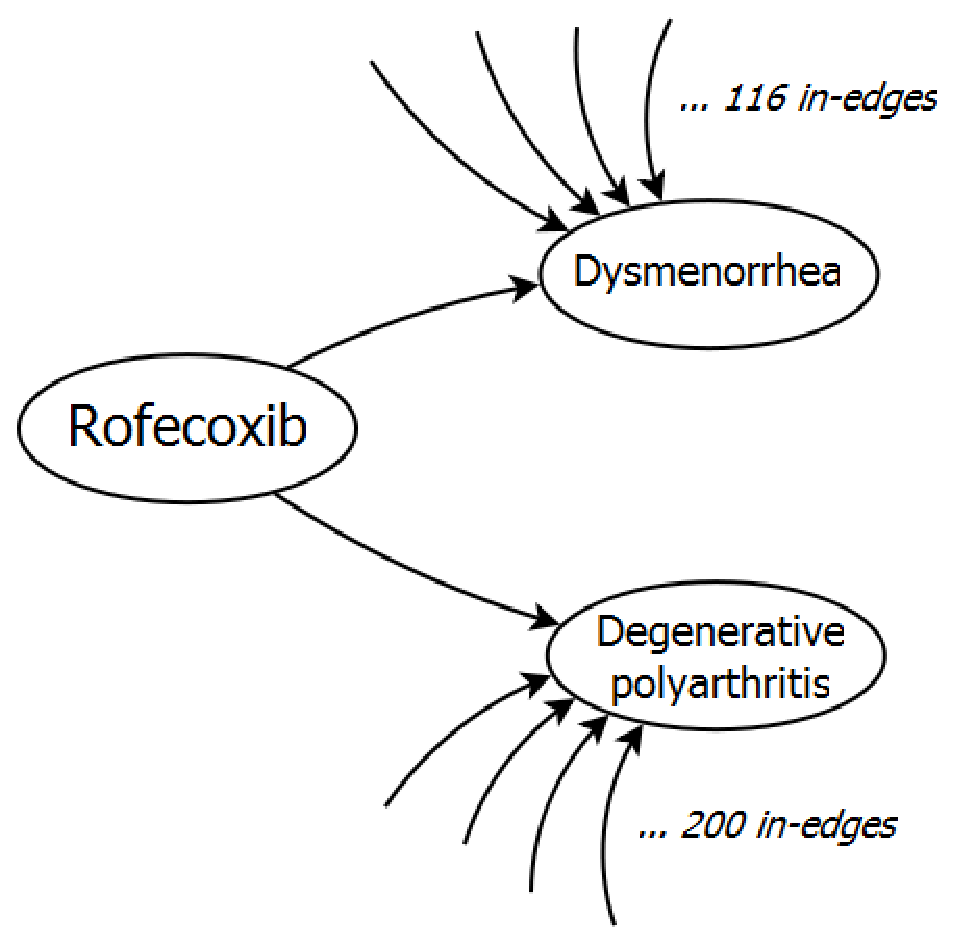
\includegraphics[width=.52\textwidth]{fig/may_treat.eps}
\end{minipage}
\begin{minipage}[c]{0.49\textwidth}\centering
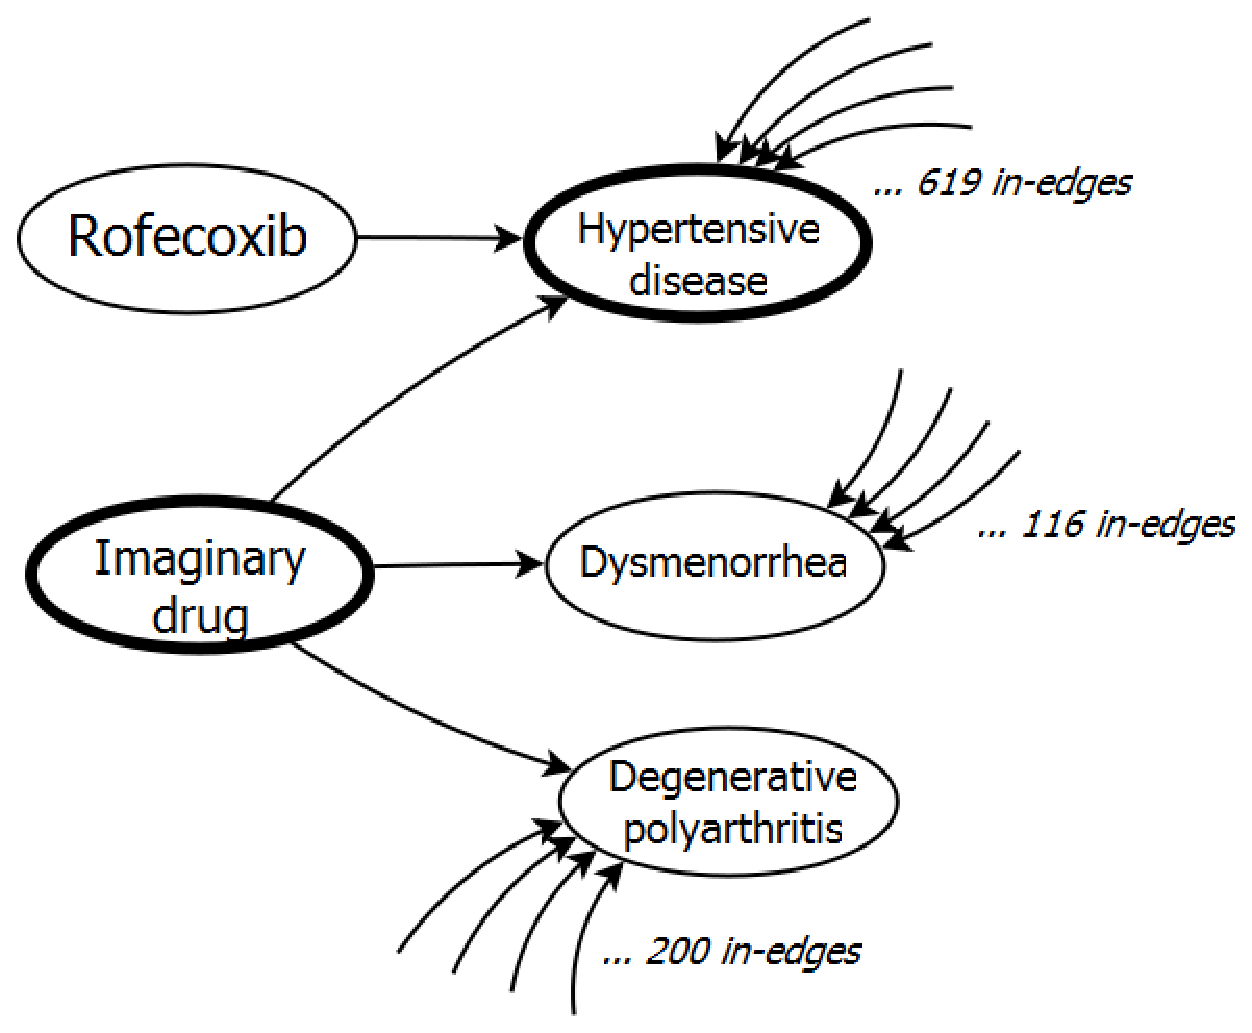
\includegraphics[width=.72\textwidth]{fig/may_treat_augmented.eps}
\end{minipage}
\caption[The may\_treat subgraph]{\label{fig:may_treat} The may\_treat subgraph before and after distortion: The left-hand side of the figure shows the may\_treat subgraph of ground truth relationships between the drug Rofecoxib and two diseases. The right-hand side shows the may\_treat subgraph with some deliberately distorted information.}
\end{figure}

\begin{table*}[tbh]\scriptsize
\begin{center}
\begin{tabular}{ c | c  c | c  c }
\hline
        &   \multicolumn{2}{c|}{w/ noisy may\_treat only}    &   \multicolumn{2}{c}{w/ data and noisy may\_treat}\\
\hline
       	&   p(\%)   &   rank    &  p(\%)    &    rank    \\
\hline
$\langle Rofecoxib, degenerative~polyarthritis\rangle$       &   3.60e-3   &   555     &   8.14e-3    &   263    \\
$\langle Rofecoxib, dysmenorrhea\rangle$    &   1.54e-2   &   246     &   1.26e-3    &   1703   \\
\hline
\end{tabular}
\end{center}
\caption[Rankings of associations on the noisy may\_treat graph]{\label{tbl:salted_may_treat}Rankings of associations on the noisy may\_treat graph (Figure~\ref{fig:may_treat} right) between Rofecoxib and two diseases derived with and without data.}
\end{table*}

Conversely, we are also interested in learning whether the data graph can help discover patterns in the ontology graph. Figure~\ref{fig:may_treat} (left) shows a subgraph of the NDFRT ``may\_treat" relationship. Rofecoxib is asserted to treat two diseases, namely, dysmenorrhea and degenerative polyarthritis. And there are altogether 116 and 200 drugs that are known to treat dysmenorrhea and degenerative polyarthritis respectively (hence the in-degrees of the nodes). Applying our method on this graph with the query term ``Rofecoxib" yields a similarity-ranked list having degenerative polyarthritis and dysmenorrhea as the top two items. Since this result is the exact ground truth, there is no improvement to be made with the incorporation of the data graph. Therefore, we alter the ground truth graph with some deliberately distorted information, as is shown in Figure~\ref{fig:may_treat} (right), so that the may\_treat graph alone produces only inferior result. More specifically, we specify that Rofecoxib should treat hypertensive disease, the very diseases that is asserted to be treated by the most drugs (a total of 619). Then we add an imaginary drug to treat degenerative polyarthritis, dysmenorrhea, and hypertensive disease. In this way, the original direct connections between Rofecoxb and degenerative polyarthritis and dysmenorrhea become erroneously indirect and are obfuscated by some the noise of high degree nodes along the path. With this scenario, we hope to learn if the incorporation of data graph can correct the misinformation in ontologies.

Table~\ref{tbl:salted_may_treat} shows the result of ranks of the associations between Rofecoxib and degenerative polyarthritis and dysmenorrhea. The ranks of the associations drastically drop to the 555th and 246th respectively on the noisy graph from the top two on the original ground truth graph. This is mainly due to the large node, hypertensive disease, in the middle of the connections. However, with the combined data and may\_treat graph, we notice that the rank of Rofecoxib and degenerative polyarthritis increases to 263rd, while the rank of Rofecoxib and  dysmenorrhea decreases to 1703rd. This shows that the data graph endorses more strongly the association between Rofecoxib and degenerative polyarthritis. Indeed, although Rofecoxib are known to treat both degenerative polyarthritis and dysmenorrhea, the former is a much more popular usage. A search on the National Library of Medicine's PubMed database\footnotemark[1] for ``Rofecoxib and polyarthritis" returns 518 results, while ``Rofecoxib and dysmenorrhea" only returns 29. This result shows that the data graph can help correct misinformation in ontologies to some extent, and in a sense, it also gives a clue of how prior beliefs fit with reality.

\footnotetext[1]{\url{http://www.ncbi.nlm.nih.gov/}}

